\documentclass[border=15pt, multi, tikz]{standalone}
\usepackage{import}
\subimport{./layers/}{init}
\usetikzlibrary{positioning}
\usetikzlibrary{3d} %for including external image 

\def\ConvColor{rgb:yellow,5;red,2.5;white,5}
\def\ConvReluColor{rgb:yellow,5;red,5;white,5}
\def\PoolColor{rgb:red,1;black,0.3}
\def\DcnvColor{rgb:blue,5;green,2.5;white,5}
\def\SoftmaxColor{rgb:magenta,5;black,7}
\def\SumColor{rgb:blue,5;green,15}
\def\BallColor{rgb:blue,5;green,2.5;white,5}
\def\verdognolo{rgb:green,5;white,2}

\begin{document}
\begin{tikzpicture}
\tikzstyle{connection}=[ultra thick,every node/.style={sloped,allow upside down},draw=\edgecolor,opacity=0.7]
%%%%%%%%%%%%%%%%%%%%%%%%%%%%%%%%%%%%%%%%%%%%%%%%%%%%%%%%%%%%%%%%%%%%%%%%%%%%%%%%%%%%%%%%
%% Draw Layer Blocks
%%%%%%%%%%%%%%%%%%%%%%%%%%%%%%%%%%%%%%%%%%%%%%%%%%%%%%%%%%%%%%%%%%%%%%%%%%%%%%%%%%%%%%%%
\node[canvas is xy plane at z=0] (ap) at (-9,0,0) {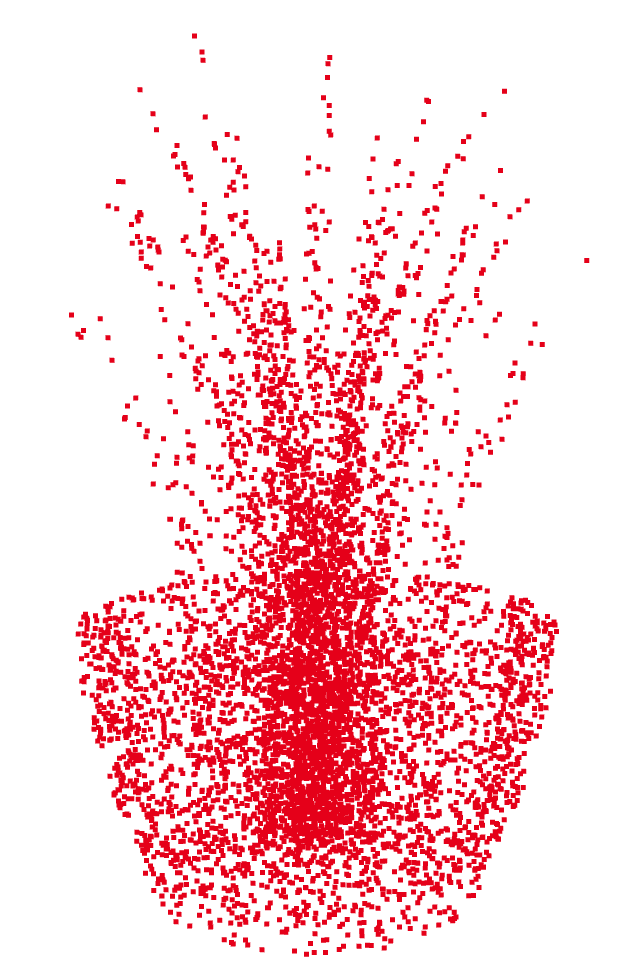
\includegraphics[width=0.4\textwidth]{all_points.png}};
\node[canvas is xy plane at z=0] (ds) at (-4,0,0) {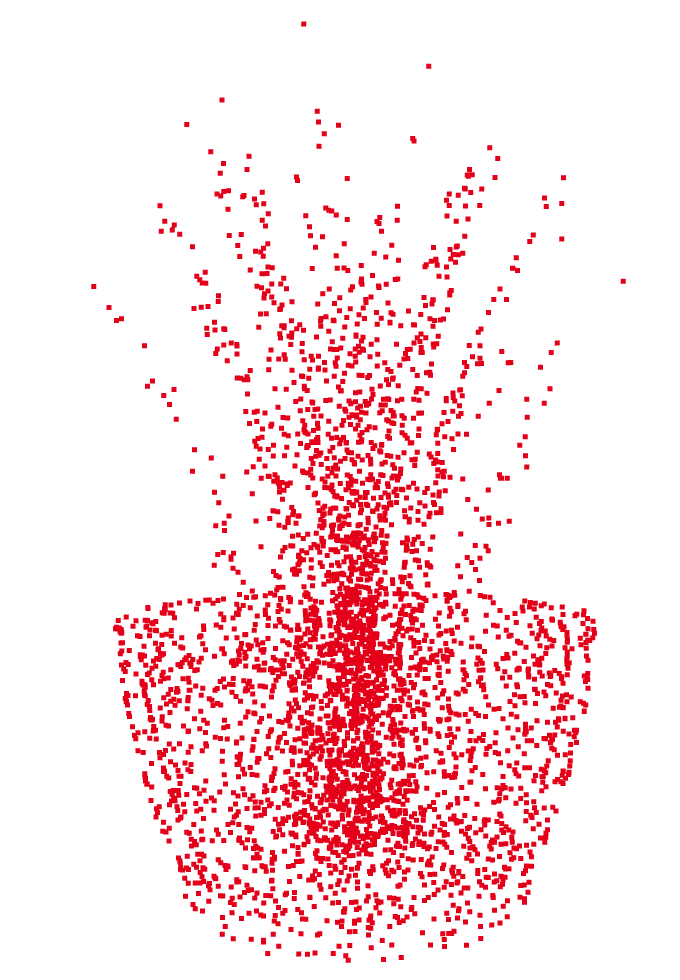
\includegraphics[width=0.45\textwidth]{downsampled.png}}
;



% conv1_1,conv1_2,%pool1
\pic[shift={(0,0,0)}] at (0,0,0) {RightBandedBox={name=cr1,caption=conv1,%
        xlabel={{" ","1@4000x3"}},ylabel=kernel 1x3,fill=\ConvColor,
        bandfill=\ConvReluColor,%
        height=30,width={0, 3},depth=20}};

%\pic[shift={(-5,-8,0)}] at (cr1-west) 
 %{Ball={name=ballsex, caption= sex,%
%fill=\verdognolo,opacity=0.7,%
 %       radius=3.5, logo=$S$}};

 % \pic[shift={(2,0,0)}] at (ballsex-east) {Box={name=dsex,caption=dense,%
     %    xlabel = {" ","32x1"}, fill=\DcnvColor, opacity=0.5,%
    %     height=2, width={0,5},depth=20}};
 


        
%\pic[shift={(0,0,0)}] at (cr1-east) {Box={name=p1,%
 %      fill=\PoolColor,opacity=0.5,height=35,width=1,depth=35}};
        
% conv2_1,conv2_2,pool2
\pic[shift={(1.5,0,0)}] at (cr1-east) {RightBandedBox={name=cr2,caption=conv2,%
        xlabel={{" "," "," "," "," "," "," ","64@4000x1"," "," "," "," "," "," "," "," ", " " }},
        zlabel= kernel 1x1,fill=\ConvColor,bandfill=\ConvReluColor,%
        height=30,width={1,1,1,1,1,1,1,1,1,1,1,1,1,1,1,1},depth=10}};
        
%\pic[shift={(0,0,0)}] at (cr2-east) {Box={name=p2,%
 %      fill=\PoolColor,opacity=0.5,height=30,width=1,depth=30}};
 
 
% conv3_1,conv3_2,pool3
\pic[shift={(1,0,0)}] at (cr2-east) {RightBandedBox={name=cr3,caption=conv3,%
        xlabel={{" "," "," "," "," "," "," ","64@4000x1"," "," "," "," "," "," "," "," ", " "}},
        zlabel=kernel 1x1,fill=\ConvColor,bandfill=\ConvReluColor,%
        height=30,width={1,1,1,1,1,1,1,1,1,1,1,1,1,1,1,1},depth=10}};
%\pic[shift={(0,0,0)}] at (cr3-east) {Box={name=p3,%
 %      fill=\PoolColor,opacity=0.5,height=23,width=1,depth=23}};
        
% conv4_1,conv4_2,conv4_3,pool4
\pic[shift={(1.2,0,0)}] at (cr3-east) {RightBandedBox={name=cr4,caption=conv4,%
        xlabel={{" "," "," "," "," "," "," ","64@4000x1"," "," "," "," "," "," "," "," ", " "}},
        zlabel=kernel 1x1,fill=\ConvColor,bandfill=\ConvReluColor,%
        height=30,width={1,1,1,1,1,1,1,1,1,1,1,1,1,1,1,1},depth=10}};
        
%\pic[shift={(0,0,0)}] at (cr4-east) {Box={name=p4,%
 %      fill=\PoolColor,opacity=0.5,height=15,width=1,depth=15}};
 
% conv5_1,conv5_2,conv5_3,pool5
\pic[shift={(1,0,0)}] at (cr4-east) {RightBandedBox={name=cr5,caption=conv5,%
        xlabel={{" "," "," "," "," "," "," "," "," "," "," "," "," "," "," ","128@4000x1"," "," "," "," "," "," "," "," "," "," "," "," "," "," "," ", " "}},
        zlabel=kernel 1x1,fill=\ConvColor,bandfill=\ConvReluColor,%
        height=30,,width={1,1,1,1,1,1,1,1,1,1,1,1,1,1,1,1,1,1,1,1,1,1,1,1,1,1,1,1,1,1,1,1},depth=10}};
        
\pic[shift={(1,0,0)}] at (cr5-east) {Box={name=p1, caption=MaxPool,%
        xlabel = {" "," "}, fill=\PoolColor,opacity=0.5,%
        height=30,width={0,2},depth=10}};    

 

\pic[shift={(1.8,0,0)}] at (p1-east) {Box={name=fl1,caption=reshape,% 
        xlabel = {" ","1024x1"}, fill=\verdognolo, opacity=0.5,%
        height=2.2, width={0,5},depth=30}};

\pic[shift={(1.5,0,0)}] at (fl1-east) {Box={name=d1,caption=dense1,%
        xlabel = {" ","1024x1"}, fill=\DcnvColor, opacity=0.5,%
        height=2, width={0,5},depth=30}};

 \pic[shift={(1.5,0,0)}] at (d1-east) {Box={name=d2,caption=dense2,%
        xlabel = {" ","512x1"}, fill=\DcnvColor, opacity=0.5,%
        height=2, width={0,5},depth=15}};

 \pic[shift={(1.5,0,0)}] at (d2-east) {Box={name=d3,caption=dense3,%
        xlabel = {" ","256x1"}, fill=\DcnvColor, opacity=0.5,%
        height=2, width={0,5},depth=7.5}};

 \pic[shift={(1.5,0,0)}] at (d3-east) {Box={name=class1,caption=,%
        xlabel = {" "," "}, fill=\SoftmaxColor, opacity=0.5,%
        height=2, width={0,2},depth=2}};

 \pic[shift={(1.5,0.5,0)}] at (d3-east) {Box={name=class2,caption=,%
        xlabel = {" "," "}, fill=\SoftmaxColor, opacity=0.5,%
        height=2, width={0,2},depth=2}};

 \pic[shift={(1.5,1,0)}] at (d3-east) {Box={name=class3,caption=,%
        xlabel = {" "," "}, fill=\SoftmaxColor, opacity=0.5,%
        height=2, width={0,2},depth=2}};

 \pic[shift={(1.5,1.5,0)}] at (d3-east) {Box={name=class4,caption=,%
        xlabel = {" "," "}, fill=\SoftmaxColor, opacity=0.5,%
        height=2, width={0,2},depth=2}};

 \pic[shift={(1.5,-0.5,0)}] at (d3-east) {Box={name=class5,caption=,%
        xlabel = {" "," "}, fill=\SoftmaxColor, opacity=0.5,%
        height=2, width={0,2},depth=2}};

 \pic[shift={(1.5,-1,0)}] at (d3-east) {Box={name=class6,caption=,%
        xlabel = {" "," "}, fill=\SoftmaxColor, opacity=0.5,%
        height=2, width={0,2},depth=2}};

 \pic[shift={(1.5,-1.5,0)}] at (d3-east) {Box={name=class7,caption=,%
        xlabel = {" "," "}, fill=\SoftmaxColor, opacity=0.5,%
        height=2, width={0,2},depth=2}};

 \pic[shift={(1.5,3,0)}] at (d3-east) {Box={name=class8,caption=,%
        xlabel = {" "," "}, fill=\SoftmaxColor, opacity=0.5,%
        height=2, width={0,2},depth=2}};

 \pic[shift={(1.5,-3,0)}] at (d3-east) {Box={name=class9,caption=40 Classes,%
        xlabel = {" "," "}, fill=\SoftmaxColor, opacity=0.5,%
        height=2, width={0,2},depth=2}};


%%%%%%%%%%%%%%%%%%%%%%%%%%%%%%%%%%%%%%%%%%%%%%%%%%%%%%%%%%%%%%%%%%%%%%%%%%%%%%%%%%%%%%%%

%%%%%%%%%%%%%%%%%%%%%%%%%%%%%%%%%%%%%%%%%%%%%%%%%%%%%%%%%%%%%%%%%%%%%%%%%%%%%%%%%%%%%%%%%    
%%% Output
%%%%%%%%%%   
%% score17
%\pic[shift={(-5,-8,0)}] at (fl1-west) {Box={name=score1,%
 %          fill=\ConvColor,%
  %        height=0,width=0,depth=0}};





%%%%%%%%%%   
%% dense2 
 %\pic[shift={(2.,0,0)}] at (d1-east) 
 %{Ball={name=d2, caption= dense2,%
%fill=\DcnvColor,opacity=0.5,%
 %       radius=2.5, logo=$1$}};
 


        
%%%%%%%%%%%%%%%%%%%%%%%%%%%%%%%%%%%%%%%%%%%%%%%%%%%%%%%%%%%%%%%%%%%%%%%%%%%%%%%%%%%%%%%%
%% Draw connections
%%%%%%%%%%%%%%%%%%%%%%%%%%%%%%%%%%%%%%%%%%%%%%%%%%%%%%%%%%%%%%%%%%%%%%%%%%%%%%%%%%%%%%%%
\draw [connection]  (cr1-east)    -- node {\midarrow} (cr2-west);
\draw [connection]  (cr2-east)    -- node {\midarrow} (cr3-west);
\draw [connection]  (cr3-east)    -- node {\midarrow} (cr4-west);
\draw [connection]  (cr4-east)    -- node {\midarrow} (cr5-west);
\draw [connection]  (cr5-east)    -- node {\midarrow} (p1-west);
\draw [connection]  (p1-east)    -- node {\midarrow} (fl1-west);
\draw [connection]  (fl1-east)    -- node {\midarrow} (d1-west);

\draw [connection]  (d1-east) -- node {\midarrow} (d2-west);
\draw [connection]  (d2-east) -- node {\midarrow} (d3-west);

\draw [connection]  (d3-east) -- node {\midarrow} (class1-west);



 %\draw [connection]  (ballsex-east) -- node {\midarrow} (dsex-west);
 %\draw [connection]  (dsex-east) -- node {\midarrow} (score1-west);

 %\draw [connection]  (score1-east) -- node {\midarrow} (fakeball-south);

%\path (p4-east) -- (cr5-west) coordinate[pos=0.25] (between4_5) ;
%\draw [connection]  (between4_5)    -- node {\midarrow} (score16-west-|between4_5) -- node {\midarrow} (score16-west);
%\draw [connection]  (d32-east) -- node {\midarrow} (elt1-west);
%\draw [connection]  (score16-east) -- node {\midarrow} (score16-east -| elt1-south) -- node {\midarrow} (elt1-south);
%\draw [connection]  (elt1-east) -- node {\midarrow} (d16-west);

%\path (p3-east) -- (cr4-west) coordinate[pos=0.25] (between3_4) ;
%\draw [connection]  (between3_4) -- node {\midarrow} (score8-west-|between3_4) -- node {\midarrow} (score8-west);
%\draw [connection]  (d16-east) -- node {\midarrow} (elt2-west);
%\draw [connection]  (score8-east) -- node {\midarrow} (score8-east -| elt2-south)-- node {\midarrow} (elt2-south);
%\draw [connection]  (elt2-east) -- node {\midarrow} (d8-west);
%\draw [connection] (d8-east) -- node{\midarrow} (softmax-west);
%%%%%%%%%%%%%%%%%%%%%%%%%%%%%%%%%%%%%%%%%%%%%%%%%%%%%%%%%%%%%%%%%%%%%%%%%%%%%%%%%%%%%%%%

\end{tikzpicture}
\end{document}\grid